\section{\label{sec:intro} Introduction}
%\gn{The new title is long and a little awkward. I actually still like ``Differential Data Selection'' or ``Differential Adaptive Data Weighting,'' what's the benefit of this new one over the previous ones?}

%\gn{I think now the intro is trying too hard to position our work in previous work, as opposed to getting across the main point. We can discuss the fine-grained differences with all of these methods in a related work section, but it'll be important to not overwhelm the readers with information before they can even understand the main point of our paper. I think the previous intro was pretty good in general, but might need to be a little bit modified to cover the most relevant recent works (e.g. \cite{learn_to_teach}).}

%\gn{``Optimizing Training'' in the title is a bit vague. ``Learning to Train Models'' might be better. Just ``Differentiable Data Selection'' may also be good?}

%To train a deep learning model, the standard method is to perform uniform stochastic gradient update steps on batches of training data. However, the data provided can have different quality, structure or domain properties from the test data, which might even deteriorate the model performance. 
While deep learning models are remarkably good at fitting large data sets, their performance is also highly sensitive to the structure and domain of their training data. Training on out-of-domain data can lead to worse model performance, while using more relevant data can assist transfer learning.
%\gn{This comment was commented out, but I still think it's relevant. What problems result from this sensitivity to quality or structural domain properties? For example, ``leading to lower performance when training sets are noisy or out-of-domain''?}
Previous work has attempted to create strategies to handle this sensitivity by selecting subsets of the data to train the model on \citep{jiang-zhai-2007-instance,wang-etal-2017-instance,axelrod2011domain,moore2010intelligent}, providing different weights for each example \citep{importance_weight,learn_reweight}, or changing the presentation order of data \citep{cl_bengio,rl_nmt}.
%Many prior work strive to improve model performance by designing better data usage strategies.
%Research on data filtering has found that removing noisy data, or selecting in-domain or structurally similar data can lead to large improvements in model performance while potentially reducing the training time~\citep{jiang-zhai-2007-instance,wang-etal-2017-instance,axelrod2011domain,foster-etal-2010-discriminative,moore2010intelligent,learn_reweight}.
%Curriculum learning, on the other hand, improves the model performance by presenting the model easy examples first and then moving towards harder examples~\citep{cl_bengio}.
%More broadly, good data usage strategies can benefit transfer learning, where we want to use data from a resource rich task/domain to improve the target task/domain we are interested in.
%For example, while training on data from related high-resource languages is an effective approach for improve the model performance on low-resource languages, identifying the good related languages to use is crucial for a competitive model~\citep{TCS}.   

However, there are several challenges with the existing work on better data usage strategies. Most work data filtering criterion or training curriculum rely on domain-specific knowledge and hand-designed heuristics, which can be sub-optimal. To avoid hand designed heuristics, several works propose to optimize a parameterized neural network to learn the data usage schedule, but most of them are tailored to specific use cases, such as handling noisy data for classification~\citep{mentornet}, learning a curriculum learning strategy for NMT~\citep{rl_nmt}, and actively selecting data for annotation~\citep{learn_active_learn,reinforce_cotrain}.
%\gn{What specific use cases? Just saying ``specific'' doesn't give readers an idea how sub-optimal they are.}.
\cite{learn_to_teach} proposes a more general teacher-student framework that first trains a teacher network to select data that directly optimizes development set accuracy over multiple training runs.
% to determine the training decisions of the student model, including optimizer choice and data filtering choice etc. They optimize the data filtering network with Reinforcement Learning~(RL) using the change in dev set loss as the reward for selecting a data instance.
However, because running multiple runs of training simply to train this teacher network entails an $n$-fold increase in training time for $n$ runs, this is infeasible in many practical settings.
In addition, in preliminary experiments we also found the single reward signal provided by dev set accuracy at the end of training noisy to the extent that we were not able to achieve results competitive with simpler heuristic training methods.


%\gn{I made significant changes here, importantly including citing \cite{learn_reweight}. If there's highly relevant work, it's not very honest to not cite it in the introduction, so I added it here and noted that it has been used for filtering noisy examples. Later in the paper we can explain the differences in more detail, then in the experiments we can note that we beat it handily.}
In this paper, we propose an alternative: a general Reinforcement Learning~(RL) framework for optimizing training data usage by training a \emph{scorer network} that minimizes the model loss on the development set.
We formulate the scorer network as a function of the current training examples only,
%\gn{``training data only'' could be ``current training example''?}
making it possible to re-use the model architecture which is designed and trained for the main task. Thus, our method requires no heuristics and is generalizable to various tasks. To make the scorer adaptive, we perform frequent and efficient updates of the scorer network using a reward function inspired by recent work on learning using data from auxiliary tasks~\citep{cos_sim,meta_aux_learn}, which use the similarity between two gradients as a measure of task relevance.
We propose to use the gradient alignment between the training examples and the dev set as a reward signal for \emph{a parametric scorer network}, as illustrated in Figure \ref{fig:method}. We then formulate our framework as an optimization problem found in many prior works such as meta-learning~\citep{finn2017model}, noisy data filtering~\citep{learn_reweight}, and neural architecture search~\citep{darts}, and demonstrate that our proposed update rules follow a direct differentiation of the scorer parameters to optimize the model loss on the dev set.
Thus we refer to our framework as ``Differentiable Data Selection''~(\dds).

%\begin{wrapfigure}{r}{0.5\textwidth}
\begin{figure}
    \centering
    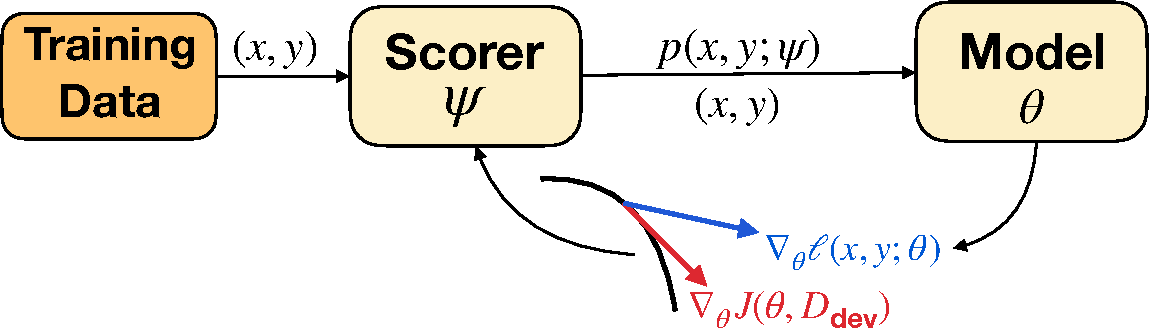
\includegraphics[width=0.4\textwidth]{figs/method_plot_crop.pdf}
    \caption{The general workflow of \dds.}
    \label{fig:method}
\end{figure}
%\end{wrapfigure}

We demonstrate two concrete instantiations of the \dds~framework, one for a more general case of image classification, and the other for a more specific case of neural machine translation~(NMT). For image classification, we test on both CIFAR-10 and ImageNet. For NMT, we focus on a multilingual setting, where we optimize data usage from a multilingual corpus to improve the performance on a particular language. % Our contributions are: 1) we propose a general and efficient framework for optimizing training data usage using a teacher network; 2) we provide two specific algorithms for
For these two very different and realistic tasks, we find the \dds~framework brings significant improvements over the baselines for all settings.